\documentclass{article}
\usepackage{tikz}
\usepackage{amssymb}
\usepackage{amsmath} % pour array
\usepackage{xcolor}

% Définitions des couleurs utilisées
\definecolor{mycol}{rgb}{1,0,0}
\definecolor{mycol2}{rgb}{0.5,0.5,0.5}
\definecolor{mycol3}{rgb}{0.4,0,0.8}
\definecolor{mycol4}{rgb}{1,0.9,0}

\begin{document}
	
	\begin{center}
		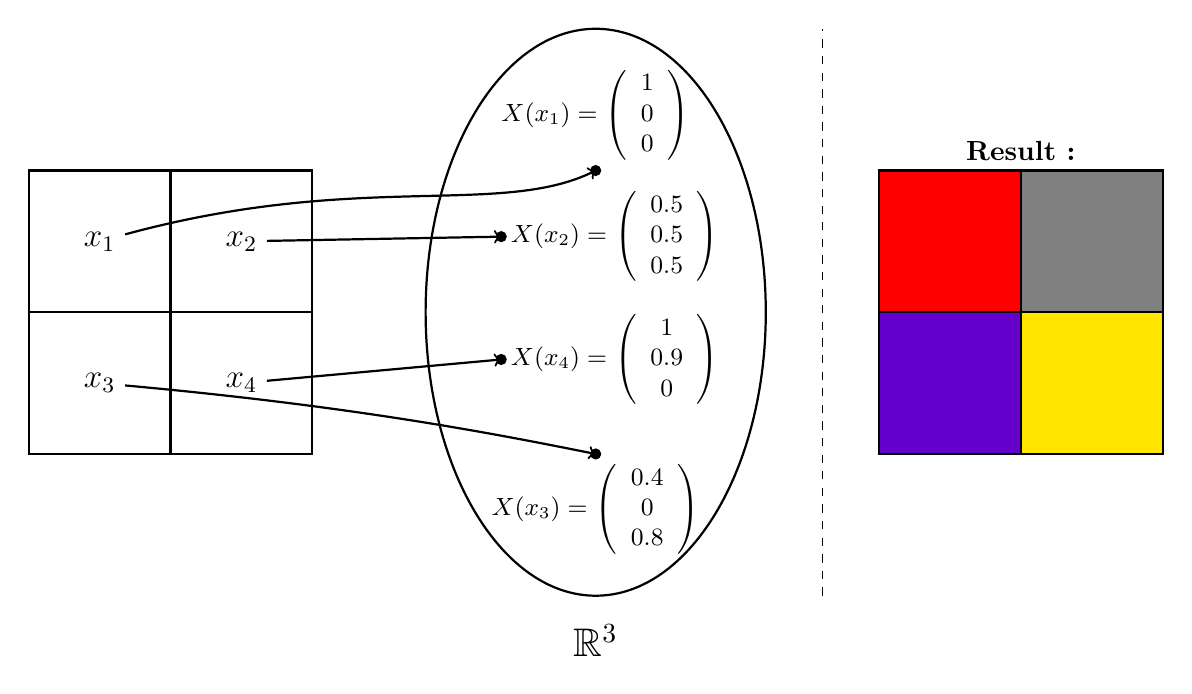
\begin{tikzpicture}[scale=1.2]
			
			% Carré à gauche (3x3)
			\draw[thick] (-6,-1.5) rectangle (-3,1.5);
			\draw[thick] (-4.5,-1.5) -- (-4.5,1.5); % division verticale
			\draw[thick] (-6,0) -- (-3,0);          % division horizontale
			
			% Noms des variables dans le carré gauche
			\node (x1) at (-5.25, 0.75) {\large $x_1$};
			\node (x2) at (-3.75, 0.75) {\large $x_2$};
			\node (x3) at (-5.25, -0.75) {\large $x_3$};
			\node (x4) at (-3.75, -0.75) {\large $x_4$};
			
			% Ellipse au centre
			\draw[thick] (0, 0) ellipse (1.8 and 3);
			\node[below] at (0,-3.2) {\Large $\mathbb{R}^3$};
			
			% Carré à droite (3x3) avec couleurs dans chaque sous-partie
			\fill[mycol]   (3,0) rectangle (4.5,1.5);
			\fill[mycol2]  (4.5,0) rectangle (6,1.5);
			\fill[mycol3]  (3,-1.5) rectangle (4.5,0);
			\fill[mycol4]  (4.5,-1.5) rectangle (6,0);
			
			\draw[thick] (3,-1.5) rectangle (6,1.5);
			\draw[thick] (4.5,-1.5) -- (4.5,1.5);   % division verticale
			\draw[thick] (3,0) -- (6,0);            % division horizontale
			
			% Texte au-dessus du carré de droite
			\node[above] at (4.5,1.5) {\textbf{Result :}};
			
			% Trait pointillé entre ellipse et carré de droite
			\draw[dashed] (2.4,-3) -- (2.4,3);
			
			% Points d'arrivée (petits) dans l'ellipse avec labels au-dessus ou en dessous selon la position
			\filldraw[black] (0,1.5) circle (1.5pt) node[anchor=south] {\small $X(x_1) = \left(\begin{array}{c} 1 \\ 0 \\ 0 \end{array}\right)$};
			\filldraw[black] (-1,0.8) circle (1.5pt) node[anchor=west] {\small $X(x_2) = \left(\begin{array}{c} 0.5 \\ 0.5 \\ 0.5 \end{array}\right)$};
			\filldraw[black] (0,-1.5) circle (1.5pt) node[anchor=north] {\small $X(x_3) = \left(\begin{array}{c} 0.4 \\ 0 \\ 0.8 \end{array}\right)$};
			\filldraw[black] (-1,-0.5) circle (1.5pt) node[anchor=west] {\small $X(x_4) = \left(\begin{array}{c} 1 \\ 0.9 \\ 0 \end{array}\right)$};
			
			% Flèches des variables vers ellipse (partent des noms)
			\draw[->, thick] (x1) .. controls (-2.5, 1.5) and (-1,1) .. (0,1.5);
			\draw[->, thick] (x2) -- (-1, 0.8);
			\draw[->, thick] (x3) .. controls (-2.5,-1) and (-1,-1.3) .. (0,-1.5);
			\draw[->, thick] (x4) -- (-1,-0.5);
			
		\end{tikzpicture}
	\end{center}
	
\end{document}